%%%%%%%%%%%%%%%%%%%%%%%%%%%%%%%%%%%%%%%%%
% Beamer Presentation
% LaTeX Template
% Version 1.0 (10/11/12)
%
% This template has been downloaded from:
% http://www.LaTeXTemplates.com
%
% License:
% CC BY-NC-SA 3.0 (http://creativecommons.org/licenses/by-nc-sa/3.0/)
%
%%%%%%%%%%%%%%%%%%%%%%%%%%%%%%%%%%%%%%%%%

%----------------------------------------------------------------------------------------
%	PACKAGES AND THEMES
%----------------------------------------------------------------------------------------

\documentclass{beamer}

\mode<presentation> {

% The Beamer class comes with a number of default slide themes
% which change the colors and layouts of slides. Below this is a list
% of all the themes, uncomment each in turn to see what they look like.

%\usetheme{default}
%\usetheme{AnnArbor}
%\usetheme{Antibes}
%\usetheme{Bergen}
%\usetheme{Berkeley}
%\usetheme{Berlin}
%\usetheme{Boadilla}
%\usetheme{CambridgeUS}
%\usetheme{Copenhagen}
\usetheme{Darmstadt}
%\usetheme{Dresden}
%\usetheme{Frankfurt}
%\usetheme{Goettingen}
%\usetheme{Hannover}
%\usetheme{Ilmenau}
%\usetheme{JuanLesPins}
%\usetheme{Luebeck}
%\usetheme{Madrid}
%*\usetheme{Malmoe}
%\usetheme{Marburg}
%\usetheme{Montpellier}
%\usetheme{PaloAlto}
%\usetheme{Pittsburgh}
%\usetheme{Rochester}
%\usetheme{Singapore}
%\usetheme{Szeged}
%\usetheme{Warsaw}

% As well as themes, the Beamer class has a number of color themes
% for any slide theme. Uncomment each of these in turn to see how it
% changes the colors of your current slide theme.

%\usecolortheme{albatross}
%\usecolortheme{beaver}
%\usecolortheme{beetle}
%\usecolortheme{crane}
%\usecolortheme{dolphin}
%\usecolortheme{dove}
%\usecolortheme{fly}
%\usecolortheme{lily}
\usecolortheme{orchid}
%\usecolortheme{rose}
%\usecolortheme{seagull}
%\usecolortheme{seahorse}
%\usecolortheme{whale}
%\usecolortheme{wolverine}

%\setbeamertemplate{footline} % To remove the footer line in all slides uncomment this line
%\setbeamertemplate{footline}[page number] % To replace the footer line in all slides with a simple slide count uncomment this line

%\setbeamertemplate{navigation symbols}{} % To remove the navigation symbols from the bottom of all slides uncomment this line
}


\usepackage{graphicx} % Allows including images
\usepackage{booktabs} % Allows the use of \toprule, \midrule and \bottomrule in tables
\usepackage{xspace}
\usepackage{caption}
\usepackage{subfigure}
\usepackage[english,brazil]{babel}
\usepackage[utf8]{inputenc}

%Renomeia o nome padrao das figuras.
\renewcommand{\figurename}{Figura}
\renewcommand{\tablename}{Tabela}
%----------------------------------------------------------------------------------------
%	TITLE PAGE
%----------------------------------------------------------------------------------------

\title[Computação Gráfica]{Transformações 2D} % The short title appears at the bottom of every slide, the full title is only on the title page

\author{Uéliton Freitas} % Your name
\institute[UFMS] % Your institution as it will appear on the bottom of every slide, may be shorthand to save space
{
Universidade Católica Don Bosco - UCDB \\ % Your institution for the title page
\medskip
\textit{freitas.ueliton@gmail.com} % Your email address
}
\date{\today} % Date, can be changed to a custom date


\begin{document}

\begin{frame}
\titlepage % Print the title page as the first slide
\end{frame}

\begin{frame}
\frametitle{Sumário} % Table of contents slide, comment this block out to remove it
\tableofcontents % Throughout your presentation, if you choose to use \section{} and \subsection{} commands, these will automatically be printed on this slide as an overview of your presentation
\end{frame}




%----------------------------------------------------------------------------------------
%	PRESENTATION SLIDES
%----------------------------------------------------------------------------------------

%------------------------------------------------
\section{Introdução} 
%------------------------------------------------

%\section{Speeded-Up Robust Features - SURF} % A subsection can be created just before a set of slides with a common theme to further break down your presentation into chunks
%\section{Baf Of Features and Colors}

%\section{Refer\^encias}
%%%%%%%%%%%%%%%%%%%%%%%%%%%%%%%%%%%%%%%%%%%%%%%%%%%%%%%%%%%%%%%%%%%%%%%%%%%%%%%%%%%%%%%%%%
\begin{frame}
\frametitle{Introdução}


	\begin{block}{Transformações Geométricas}
		\begin{itemize}
			\item São transformações aplicadas aos modelos de objetos:
				\begin{itemize}
					\item Posicionamento (translação).
					\item Orientação (rotação). 
					\item Tamanho (escala).
					\item Reflexão.
					\item Crisalhamento.
				\end{itemize}
		\end{itemize}
	\end{block}
	
\end{frame}

%%%%%%%%%%%%%%%%%%%%%%%%%%%%%%%%%%%%%%%%%%%%%%%%%%%%%%%%%%%%%%%%%%%%%%%%%%%%%%%%%%%%%%%%%%
\section{Operações Básicas}
\begin{frame}
\frametitle{Transformações de Corpos Rígidos}


	\begin{block}{Transformações de Corpo Rígido}
		\begin{itemize}
			\item São transformações que não alteram as dimensões dos objetos:
				\begin{itemize}
					\item Posicionamento (translação).
					\item Orientação (rotação).
				\end{itemize}
			\item Mantém as distâncias e ângulos do objeto.
		\end{itemize}
	\end{block}
	
\end{frame}

%%%%%%%%%%%%%%%%%%%%%%%%%%%%%%%%%%%%%%%%%%%%%%%%%%%%%%%%%%%%%%%%%%%%%%%%%%%%%%%%%%%%%%%%%%

\subsection{Translação}
\begin{frame}
\frametitle{Translação}


	\begin{block}{Translação de um Objeto}
		\begin{itemize}
			\item A translação consiste em adicionar uma ``variação'' as coordenadas de um objeto.
			\begin{itemize}
				\item $x' = x + \Delta x$
				\item $y' = y + \Delta y$
			\end{itemize}
		\end{itemize}
		
	\end{block}
	
\end{frame}

%%%%%%%%%%%%%%%%%%%%%%%%%%%%%%%%%%%%%%%%%%%%%%%%%%%%%%%%%%%%%%%%%%%%%%%%%%%%%%%%%%%%%%%%%%

\begin{frame}
\frametitle{Translação}
	\begin{figure}[!h]
			\begin{center}
			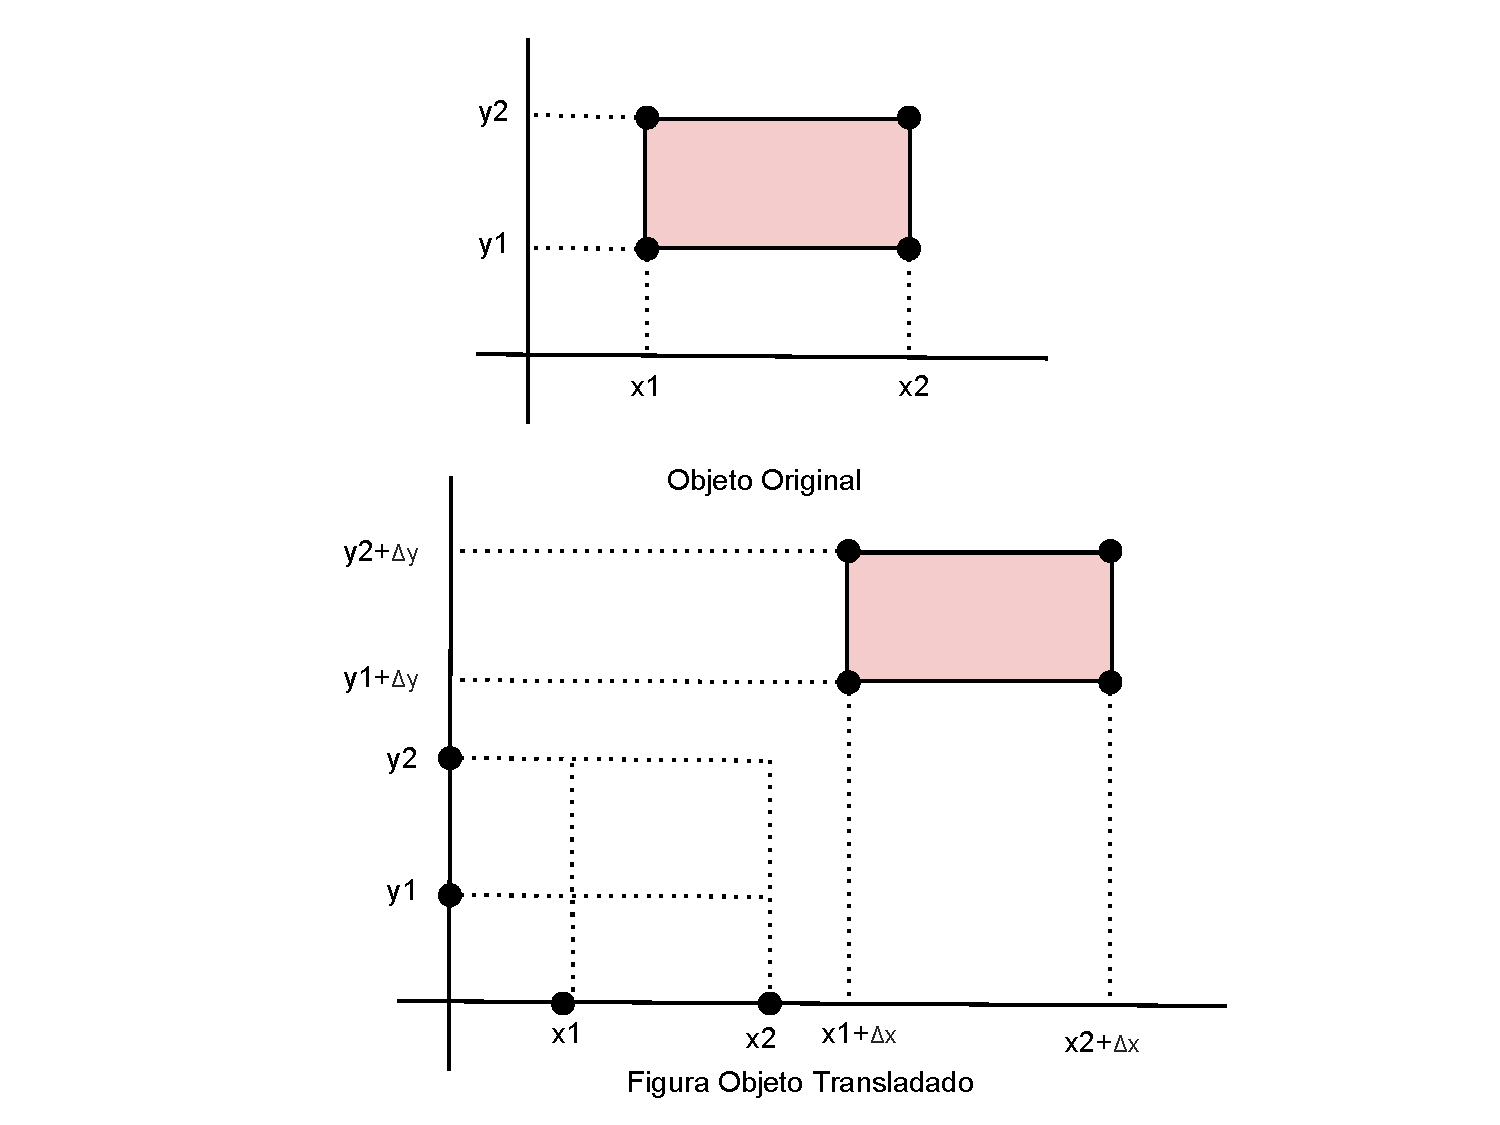
\includegraphics[width=0.9\textwidth]{Figures/Translacao}
			\end{center}
	\end{figure}	
	
\end{frame}

%%%%%%%%%%%%%%%%%%%%%%%%%%%%%%%%%%%%%%%%%%%%%%%%%%%%%%%%%%%%%%%%%%%%%%%%%%%%%%%%%%%%%%%%%%
\begin{frame}
\frametitle{Translação}


	\begin{block}{Translação de um Objeto}
		\begin{itemize}
			\item A translação consiste em adicionar uma ``variação'' as coordenadas de um objeto.
			\begin{itemize}
				\item $x' = x + \Delta x$
				\item $y' = y + \Delta y$
			\end{itemize}
		\end{itemize}
		
	\end{block}
	
	\begin{block}{Notação Matricial}
		\begin{itemize}
			\item Utilizando uma notação matricial é possível representar a operação de translação da seguinte forma:
		\end{itemize}
		\begin{eqnarray*}
			\textbf{P}' = \textbf{P} + \textbf{T} \\
			\textbf{P}' = 	\begin{bmatrix} 
								x' \\
								y' \\
							\end{bmatrix}
			,\textbf{P} = 	\begin{bmatrix}
								x \\
								y \\
							\end{bmatrix}
			,\textbf{T} = 	\begin{bmatrix}
								\Delta x \\
								\Delta y \\
							\end{bmatrix}
		\end{eqnarray*}
		
	\end{block}
	
\end{frame}

%%%%%%%%%%%%%%%%%%%%%%%%%%%%%%%%%%%%%%%%%%%%%%%%%%%%%%%%%%%%%%%%%%%%%%%%%%%%%%%%%%%%%%%%%%
\subsection{Rotação}
\begin{frame}
\frametitle{Rotação}


	\begin{block}{Rotação de um Objeto}
		\begin{itemize}
			\item Dá-se a operação de rotação de um objeto através de um \textbf{eixo de rotação} e um \textbf{ângulo de rotação}.
			\item No plano 2D, o eixo de rotação dá-se pelo eixo perpendicular ao plano $xy$.
		\end{itemize}
	\end{block}
	
	\begin{figure}[!h]
			\begin{center}
			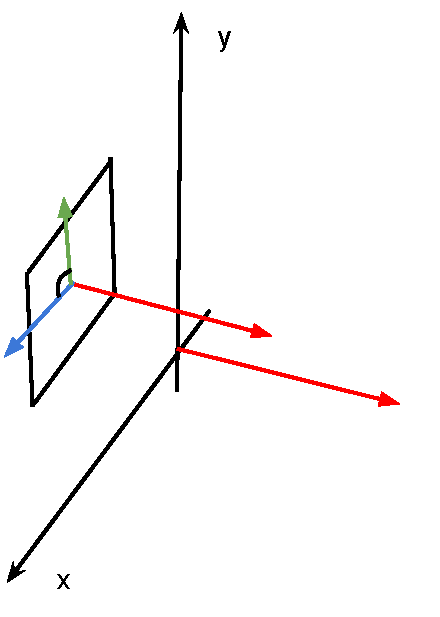
\includegraphics[width=0.3\textwidth]{Figures/EixoRotacao2D}
			\end{center}
	\end{figure}
	
\end{frame}

%%%%%%%%%%%%%%%%%%%%%%%%%%%%%%%%%%%%%%%%%%%%%%%%%%%%%%%%%%%%%%%%%%%%%%%%%%%%%%%%%%%%%%%%%%

\begin{frame}
\frametitle{Rotação}


	\begin{block}{Rotação de um Objeto}
		\begin{itemize}
			\item Para realizar a rotação de um objeto em 2D, é necessário um ângulo $\theta$ e o ponto de ponto de rotação $(x,y)$, que é o ponto de intersecção com o eixo perpendicular ao plano $xy$.
			\begin{itemize}
				\item Se $\theta > 0$, a rotação é no sentido anti-horária.
				\item Se $\theta < 0$, a rotação é no sentido horário.
			\end{itemize}
		\end{itemize}
	\end{block}
	
	\begin{figure}[!h]
			\begin{center}
			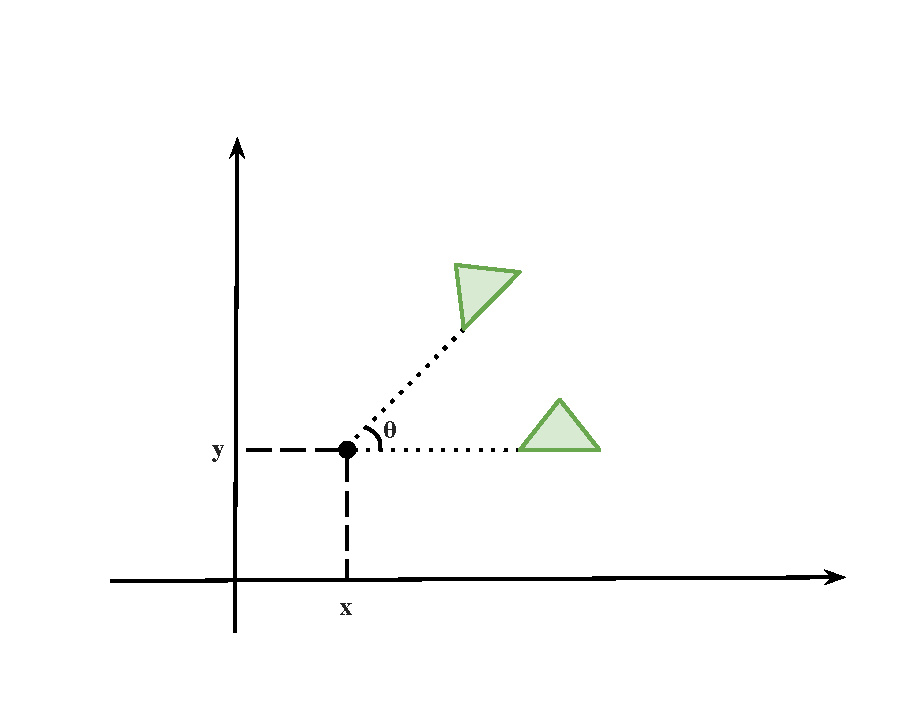
\includegraphics[width=0.5\textwidth]{Figures/ExemploRotacao}
			\end{center}
	\end{figure}
	
\end{frame}

%%%%%%%%%%%%%%%%%%%%%%%%%%%%%%%%%%%%%%%%%%%%%%%%%%%%%%%%%%%%%%%%%%%%%%%%%%%%%%%%%%%%%%%%%%

\begin{frame}
\frametitle{Rotação}


	\begin{block}{Rotação de um Objeto}
		\begin{itemize}
			\item Simplificando:
			\begin{itemize}
				\item Considera-se que o ponto de rotação está na origem.
				\item O raio $r$ é constante.
				\item $\phi$ é o ângulo do ponto $P = (x,y)$ em relação a origem.
				\item $\theta$ é o ângulo de rotação.
			\end{itemize}
		\end{itemize}
	\end{block}
	
	\begin{figure}[!h]
			\begin{center}
			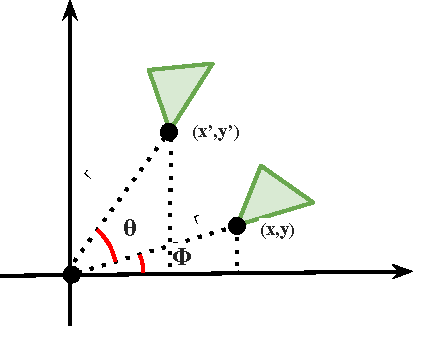
\includegraphics[width=0.5\textwidth]{Figures/ExemploRotacao2}
			\end{center}
	\end{figure}
	
\end{frame}

%%%%%%%%%%%%%%%%%%%%%%%%%%%%%%%%%%%%%%%%%%%%%%%%%%%%%%%%%%%%%%%%%%%%%%%%%%%%%%%%%%%%%%%%%%

\begin{frame}
\frametitle{Rotação}

	\begin{block}{Sabemos que:}
		\begin{itemize}
			\item $cos(\theta) = \frac{\text{Cateto adjacente}}{\text{Hipotenuza}}$
			\item $sen(\theta) = \frac{\text{Cateto oposto}}{\text{Hipotenuza}}$
		\end{itemize}
	\end{block}

	\begin{block}{Então temos que:}
		\begin{itemize}
			\item $cos(\phi + \theta) = \frac{x'}{r} \implies x' = cos(\phi + \theta)\cdot r$
			\item $sen(\phi + \theta) = \frac{y'}{r} \implies y' = sen(\phi + \theta)\cdot r$
		\end{itemize}
	\end{block}
	
\end{frame}


%%%%%%%%%%%%%%%%%%%%%%%%%%%%%%%%%%%%%%%%%%%%%%%%%%%%%%%%%%%%%%%%%%%%%%%%%%%%%%%%%%%%%%%%%%

\begin{frame}
\frametitle{Rotação}

	\begin{block}{Como:}
		\begin{itemize}
			\item $cos(\alpha + \beta) = cos(\alpha) \cdot cos(\beta) - sen(\alpha)\cdot sen(\beta)$
			\item $sen(\alpha + \beta) = cos(\alpha) \cdot sen(\beta)   + sen(\alpha)\cdot cos(\beta)$
		\end{itemize}
	\end{block}

	\begin{block}{Então temos que:}
		\begin{itemize}
			\item $ x' =  r \cdot cos(\phi) \cdot cos(\theta) - r \cdot sen(\phi) \cdot sen(\theta)$
			\item $ y' =  r \cdot cos(\phi) \cdot sen(\theta) + r \cdot sen(\phi) \cdot cos(\theta)$
		\end{itemize}
	\end{block}
	
\end{frame}

%%%%%%%%%%%%%%%%%%%%%%%%%%%%%%%%%%%%%%%%%%%%%%%%%%%%%%%%%%%%%%%%%%%%%%%%%%%%%%%%%%%%%%%%%%

\begin{frame}
\frametitle{Rotação}

	\begin{block}{Coordenadas Polares}
		\begin{itemize}
			\item<1-> Temos que $P = (x,y)$ pode ser escrito na forma de coordenadas polares:
				\begin{itemize}
					\item $x = r \cdot cos(\theta)$
					\item $y = r \cdot sen(\theta)$ 
				\end{itemize}
			\item<2-> Substituindo os valores temos:
				\begin{itemize}
					\item $x' = x \cdot cos(\theta) - y \cdot sen(\theta)$
					\item $y' = x \cdot sen(\theta) + y \cdot cos(\theta)$
				\end{itemize}
		\end{itemize}
	\end{block}
	
	\begin{block}{Em Notação de Matriz}
		\begin{eqnarray*}
			\textbf{P}' = \textbf{R} \cdot \textbf{P} \\
			\textbf{P}' = 	\begin{bmatrix} 
								x' \\
								y' \\
							\end{bmatrix}
			=
			 \begin{bmatrix}
								cos(\theta) & -sen(\theta) \\
								sen(\theta) & cos(\theta)\\
							\end{bmatrix}
			\cdot \begin{bmatrix}
								x \\
								y \\
							\end{bmatrix}
		\end{eqnarray*}
	\end{block}

	
\end{frame}


%%%%%%%%%%%%%%%%%%%%%%%%%%%%%%%%%%%%%%%%%%%%%%%%%%%%%%%%%%%%%%%%%%%%%%%%%%%%%%%%%%%%%%%%%%

\begin{frame}
\frametitle{Rotação}


	\begin{block}{Rotação de em Torno de um Ponto Arbitrário}
			\begin{itemize}
				\item Rotação em torno de um ponto $(x_r,y_r)$.
			\end{itemize}
	\end{block}
	
	\begin{figure}[!h]
			\begin{center}
			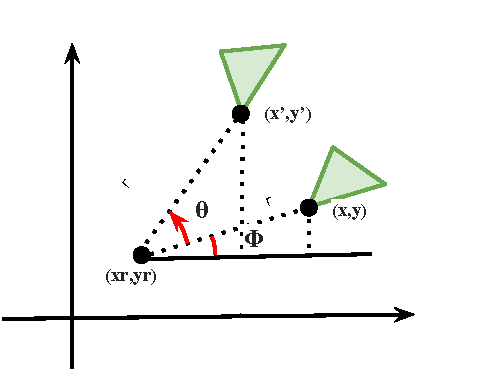
\includegraphics[width=0.5\textwidth]{Figures/ExemploRotacao3}
			\end{center}
	\end{figure}
	
	
	
\end{frame}

%%%%%%%%%%%%%%%%%%%%%%%%%%%%%%%%%%%%%%%%%%%%%%%%%%%%%%%%%%%%%%%%%%%%%%%%%%%%%%%%%%%%%%%%%%

\begin{frame}
\frametitle{Rotação}

	\begin{block}{Para encontrar $x'$:}
		\begin{itemize}
			\item $cos (\phi + \theta) = \frac{x' - x_r}{r}$
			\item $x' = r \cdot cos (\phi + \theta) + x_r $	
			\item $x' = x_r + r \cdot cos(\phi) \cdot cos (\theta) - r \cdot sen(\phi) \cdot sen(\theta)$
		\end{itemize}
	\end{block}
	
	\begin{block}{Mas temos que:}
		\begin{itemize}
			\item $cos (\phi) = \frac{x-x_r}{r}$ e $sen(\phi) =\frac{y - y_r}{r}$ 
		\end{itemize}
	\end{block}
	
	\begin{block}{Então:}
		\begin{itemize}
			\item $x' = x_r + (x - x_r) \cdot cos(\theta) - (y-y_r) \cdot sen(\theta)$
			\item $y' = y_r + (x - x_r) \cdot sen(\theta) + (y-y_r) \cdot cos(\theta)$ 
		\end{itemize}
	\end{block}
	
\end{frame}


%%%%%%%%%%%%%%%%%%%%%%%%%%%%%%%%%%%%%%%%%%%%%%%%%%%%%%%%%%%%%%%%%%%%%%%%%%%%%%%%%%%%%%%%%%

\begin{frame}
\frametitle{Rotação}
		\begin{itemize}
			\item Escrevendo a operação em notação de matriz temos:
		\end{itemize}
		\begin{eqnarray*}
			\textbf{P}' = \textbf{R} \cdot \textbf{P} + \textbf{T} \\
			\begin{bmatrix} 
								x' \\
								y' \\
							\end{bmatrix}
			=
			 \begin{bmatrix}
								cos(\theta) & -sen(\theta) \\
								sen(\theta) & cos(\theta)\\
							\end{bmatrix}
			\cdot \begin{bmatrix}
								x \\
								y \\
							\end{bmatrix}
		 	+ \begin{bmatrix}
		 		x_r-x_r \cdot cos(\theta)+y_r \cdot sen(\theta) \\
				y_r-x_r \cdot sen(\theta)-y_r \cdot cos(\theta) \\		 	
		 	\end{bmatrix}
		\end{eqnarray*}
	
\end{frame}

%%%%%%%%%%%%%%%%%%%%%%%%%%%%%%%%%%%%%%%%%%%%%%%%%%%%%%%%%%%%%%%%%%%%%%%%%%%%%%%%%%%%%%%%%%

\subsection{Escala}
\begin{frame}
\frametitle{Escala}


	\begin{block}{Escala de um Objeto}
		\begin{itemize}
			\item Utiliza-se a \textbf{escala} para aumentar o tamanho de um objeto.
			\item Multiplica-se os valores das coordenadas $x,y$ por um fator $s$:\\
				\begin{itemize}
					\item $x' = x \cdot s_x$
					\item $y' = x \cdot y_x$
				\end{itemize}
			\item Em notação matricial:\\
					\begin{eqnarray*}
							\textbf{P'} = \textbf{S} \cdot \textbf{P}  \\
							\begin{bmatrix} 
								x' \\
								y' \\
							\end{bmatrix}
							=	\begin{bmatrix}
								s_x & 0 \\
								0 & s_y\\
							\end{bmatrix}
							\cdot \begin{bmatrix}
								x \\
								y \\
							\end{bmatrix}
						\end{eqnarray*}
		\end{itemize}
	\end{block}
	
\end{frame}

%%%%%%%%%%%%%%%%%%%%%%%%%%%%%%%%%%%%%%%%%%%%%%%%%%%%%%%%%%%%%%%%%%%%%%%%%%%%%%%%%%%%%%%%%%
\begin{frame}
\frametitle{Escala}


	\begin{block}{Propriedades da Escala}
		\begin{itemize}
			\item<1-> $s_x$ e $s_y$ devem ser maiores que zero.
			\item<2-> Se $s_x > 1$ e $s_y > 1$ há um aumento do objeto.
			\item<3-> Se $s_x < 1$ e $s_y < 1$ há uma diminuição do objeto.
			\item<4-> Se $s_x  = s_y$ a escala é uniforme.
			\item<5-> Se $s_x  \neq s_y$ a escala é diferencial.
		\end{itemize}
	\end{block}
	
\end{frame}



%%%%%%%%%%%%%%%%%%%%%%%%%%%%%%%%%%%%%%%%%%%%%%%%%%%%%%%%%%%%%%%%%%%%%%%%%%%%%%%%%%%%%%%%%%
\begin{frame}
\frametitle{Escala}
	
	\begin{figure}[!h]
		\begin{center}
			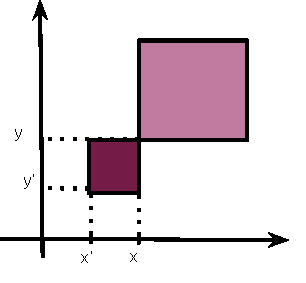
\includegraphics[width=0.5\textwidth]{Figures/Escala}
		\end{center}
		\caption{Operação de escala com $s_x = 0.5$ e $s_y = 0.5$}
	\end{figure}
	
	\begin{itemize}
		\item<2-> Pela formula atual o objeto é escalado e movido.
	\end{itemize}
	
\end{frame}

%%%%%%%%%%%%%%%%%%%%%%%%%%%%%%%%%%%%%%%%%%%%%%%%%%%%%%%%%%%%%%%%%%%%%%%%%%%%%%%%%%%%%%%%%%
\begin{frame}
\frametitle{Escala}
	
	\begin{block}{Correção da Escala de um Objeto}
		\begin{itemize}
			\item<1-> Pela formula atual o objeto é escalado e movido.
			\item<2-> Para resolver o problema do deslocamento:
				\begin{itemize}
					\item Escolha uma posição fixa $(x_f,y_f)$.
					\item Escala-se a distância entre o ponto fixo e as coordenadas do objeto.\\
				\end{itemize}
		\end{itemize}
		
		\begin{itemize}
			\item<3-> Obtemos $x'$ e $y'$ da seguinte forma:
				\begin{eqnarray*}
						x'-x_f = s_x \cdot (x - x_f) \\
						y'-y_f = s_y \cdot (y - y_f) 
				\end{eqnarray*}
			\item<4-> Assim:
				 \begin{eqnarray*}
						x'= x \cdot s_x + x_f(1 - s_x) \\
						y'= y \cdot s_y + y_f(1 - s_y)
				\end{eqnarray*}
		\end{itemize}
	\end{block}
\end{frame}


%%%%%%%%%%%%%%%%%%%%%%%%%%%%%%%%%%%%%%%%%%%%%%%%%%%%%%%%%%%%%%%%%%%%%%%%%%%%%%%%%%%%%%%%%%
\begin{frame}
\frametitle{Escala}
	
	\begin{block}{Em Notação Matricial}
		\begin{itemize}
			\item $x_f(1-s_x)$ e $y_f(1-s_y)$ são constantes para todas as coordenadas do objeto.
		\end{itemize}			
	\begin{eqnarray*}
			\textbf{P}' = \textbf{S} \cdot \textbf{P} \\
			\begin{bmatrix} 
					x' \\
					y' \\
			\end{bmatrix}
			=	\begin{bmatrix}
					s_x & 0 \\
					0 & s_y\\
					\end{bmatrix}
			\cdot \begin{bmatrix}
					x \\
					y \\
				\end{bmatrix}
			+ \begin{bmatrix}
					x_f(1-s_x) \\
					y_f(1-s_y) \\
				\end{bmatrix}
	\end{eqnarray*}
	\end{block}
	
\end{frame}

%%%%%%%%%%%%%%%%%%%%%%%%%%%%%%%%%%%%%%%%%%%%%%%%%%%%%%%%%%%%%%%%%%%%%%%%%%%%%%%%%%%%%%%%%%
\section{Coordenadas Homogêneas}
\begin{frame}
\frametitle{Coordenadas Homogêneas}
	
	\begin{block}{Coordenadas Homogêneas}
		\begin{itemize}
			\item Podem descrever objetos 2D usando matrizes $3x3$.
			\item Um ponto 2D é representado da seguinte forma utilizando coordenadas homogêneas:\\
				$P(x_h,y_h,h) = P(\frac{x}{w},\frac{y}{w},1), h \neq 0 $
			\item 	$h$ é denominado fator homogêneo, e por conveniência $ h=1$.
			\item Pode ser visto como a projeção do espaço 2D no plano $h$.
		\end{itemize}
	\end{block}
	
\end{frame}

%%%%%%%%%%%%%%%%%%%%%%%%%%%%%%%%%%%%%%%%%%%%%%%%%%%%%%%%%%%%%%%%%%%%%%%%%%%%%%%%%%%%%%%%%%

\begin{frame}
\frametitle{Coordenadas Homogêneas}
\begin{figure}[!h]
		\begin{center}
			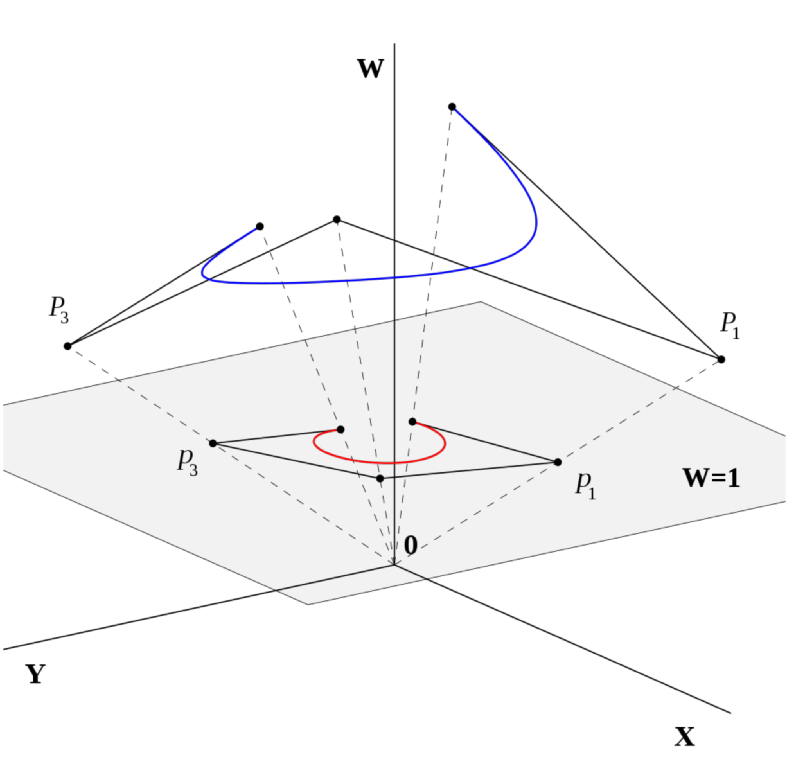
\includegraphics[width=0.5\textwidth]{Figures/coohomo}
		\end{center}
	\end{figure}
\end{frame}

%%%%%%%%%%%%%%%%%%%%%%%%%%%%%%%%%%%%%%%%%%%%%%%%%%%%%%%%%%%%%%%%%%%%%%%%%%%%%%%%%%%%%%%%%%

\begin{frame}
\frametitle{Coordenadas Homogêneas}
	\begin{block}{Coordenadas Homogêneas}
		\begin{itemize}
			\item Mas por que transformar as coordenadas 2D dos objetos em coordenadas 3D?
				\begin{itemize}
					\item<2-> Escrever as transformações como multiplicação de matrizes. 
				\end{itemize}	
		\end{itemize}
	\end{block}

\end{frame}

%%%%%%%%%%%%%%%%%%%%%%%%%%%%%%%%%%%%%%%%%%%%%%%%%%%%%%%%%%%%%%%%%%%%%%%%%%%%%%%%%%%%%%%%%%
\subsection{Translação no Sistema Homogêneo}
\begin{frame}
\frametitle{Coordenadas Homogêneas}
	\begin{block}{A Translação no Sistema Homogêneo é dada por:}
		\begin{eqnarray*}
			x_h' = 1 \cdot x_h + 0 \cdot y_h + \Delta x \cdot h \\
			y_h' = 0 \cdot x_h + 1 \cdot y_h + \Delta y \cdot h \\
			h = 0 \cdot x_h + 0 \cdot y_h + 1 \cdot h \\
		\end{eqnarray*}
	\end{block}
	
	\begin{block}{A Translação no Sistema Homogêneo em Notação de Matriz}
		\begin{eqnarray*}
			\begin{bmatrix} 
					x_h' \\
					y_h' \\
					h
			\end{bmatrix}
			=	\begin{bmatrix}
					1	& 0 	& \Delta x \\
					0 	& 1	& \Delta y \\
					0	& 0	& 1
					\end{bmatrix}
			\cdot \begin{bmatrix}
					x_h \\
					y_h \\
					h
				\end{bmatrix}
		\end{eqnarray*}
	\end{block}

\end{frame}

%%%%%%%%%%%%%%%%%%%%%%%%%%%%%%%%%%%%%%%%%%%%%%%%%%%%%%%%%%%%%%%%%%%%%%%%%%%%%%%%%%%%%%%%%%

\begin{frame}
\frametitle{Coordenadas Homogêneas}
	\begin{block}{Transformando de Volta ao Plano 2D}
		\begin{eqnarray*}
			\frac{x_h'}{h} = \frac{1 \cdot x_h + 0 \cdot y_h + \Delta x \cdot h}{h} \Rightarrow x' = x + \Delta x  \\
			\frac{y_h'}{h} = \frac{0 \cdot x_h + 1 \cdot y_h + \Delta y \cdot h}{h} \Rightarrow y' = y + \Delta y  \\
			\frac{h}{h} = \frac{0 \cdot x_h + 0 \cdot y_h + 1 \cdot h}{h} \Rightarrow h = 1  \\\\
		\end{eqnarray*}
	\end{block}


\end{frame}


%%%%%%%%%%%%%%%%%%%%%%%%%%%%%%%%%%%%%%%%%%%%%%%%%%%%%%%%%%%%%%%%%%%%%%%%%%%%%%%%%%%%%%%%%%

\begin{frame}
\frametitle{Coordenadas Homogêneas}
	\begin{block}{Matriz de Translação no Espaço 2D}
		\begin{eqnarray*}
			\textbf{P'} = \textbf{T}(\Delta x, \Delta y) \cdot \textbf{P} \\
			\begin{bmatrix} 
					x' \\
					y' \\
					1
			\end{bmatrix}
			=	\begin{bmatrix}
					1	& 0 	& \Delta x \\
					0 	& 1	& \Delta y \\
					0	& 0	& 1
					\end{bmatrix}
			\cdot \begin{bmatrix}
					x \\
					y \\
					1
				\end{bmatrix}
		\end{eqnarray*}
	\end{block}


\end{frame}


%%%%%%%%%%%%%%%%%%%%%%%%%%%%%%%%%%%%%%%%%%%%%%%%%%%%%%%%%%%%%%%%%%%%%%%%%%%%%%%%%%%%%%%%%%
\subsection{Rotação no Sistema Homogênio}
\begin{frame}
\frametitle{Coordenadas Homogêneas}
	\begin{block}{Matriz de Rotação no Espaço 2D}
		\begin{eqnarray*}
			\textbf{P'} = \textbf{R}(\theta) \cdot \textbf{P} \\
			\begin{bmatrix} 
					x' \\
					y' \\
					1
			\end{bmatrix}
			=	\begin{bmatrix}
					cos(\theta)	& -sen (\theta) 	& 0 \\
					sen(\theta)	& cos (\theta) 	& 0 \\
					0	& 0	& 1
					\end{bmatrix}
			\cdot \begin{bmatrix}
					x \\
					y \\
					1
				\end{bmatrix}
		\end{eqnarray*}
	\end{block}


\end{frame}

%%%%%%%%%%%%%%%%%%%%%%%%%%%%%%%%%%%%%%%%%%%%%%%%%%%%%%%%%%%%%%%%%%%%%%%%%%%%%%%%%%%%%%%%%%
\subsection{Escala no Sistema Homogênio}
\begin{frame}
\frametitle{Coordenadas Homogêneas}
	\begin{block}{Matriz de Escala no Espaço 2D}
		\begin{eqnarray*}
			\textbf{P'} = \textbf{S}(s_x,s_y) \cdot \textbf{P} \\
			\begin{bmatrix} 
					x' \\
					y' \\
					1
			\end{bmatrix}
			=	\begin{bmatrix}
					s_x	& 0 	& 0 \\
					0	& s_y 	& 0 \\
					0	& 0	& 1
					\end{bmatrix}
			\cdot \begin{bmatrix}
					x \\
					y \\
					1
				\end{bmatrix}
		\end{eqnarray*}
	\end{block}


\end{frame}

%%%%%%%%%%%%%%%%%%%%%%%%%%%%%%%%%%%%%%%%%%%%%%%%%%%%%%%%%%%%%%%%%%%%%%%%%%%%%%%%%%%%%%%%%%
\section{Transformações Inversas}
\begin{frame}
\frametitle{Transformações Inversas}
	\begin{block}{Inversa da Translação}
		\begin{eqnarray*}
			\textbf{P'} = \textbf{T}^{-1}(\Delta x, \Delta y) \cdot \textbf{P} \\
			\begin{bmatrix} 
					x' \\
					y' \\
					1
			\end{bmatrix}
			=	\begin{bmatrix}
					1	& 0 	& -\Delta x \\
					0 	& 1	& -\Delta y \\
					0	& 0	& 1
					\end{bmatrix}
			\cdot \begin{bmatrix}
					x \\
					y \\
					1
				\end{bmatrix}
		\end{eqnarray*}
		\begin{itemize}
			\item Basta inverter os sinais de $\Delta x$ e $\Delta y$.
		\end{itemize}
	\end{block}
\end{frame}

%%%%%%%%%%%%%%%%%%%%%%%%%%%%%%%%%%%%%%%%%%%%%%%%%%%%%%%%%%%%%%%%%%%%%%%%%%%%%%%%%%%%%%%%%%

\begin{frame}
\frametitle{Transformações Inversas}
	\begin{block}{Inversa da Rotação}
		\begin{eqnarray*}
			\textbf{P'} = \textbf{R}^{-1}(\theta) \cdot \textbf{P} \\
			\begin{bmatrix} 
					x' \\
					y' \\
					1
			\end{bmatrix}
			=	\begin{bmatrix}
					cos(\theta)	& sen (\theta) 	& 0 \\
					-sen(\theta)	& cos (\theta) 	& 0 \\
					0	& 0	& 1
					\end{bmatrix}
			\cdot \begin{bmatrix}
					x \\
					y \\
					1
				\end{bmatrix}
		\end{eqnarray*}
		\begin{itemize}
			\item Utilizado para rotacionado no sentido horário.
			\item Nete caso, $\textbf{R}^{-1} = \textbf{R}^t$.
		\end{itemize}
	\end{block}
\end{frame}


%%%%%%%%%%%%%%%%%%%%%%%%%%%%%%%%%%%%%%%%%%%%%%%%%%%%%%%%%%%%%%%%%%%%%%%%%%%%%%%%%%%%%%%%%%

\begin{frame}
\frametitle{Transformações Inversas}
	\begin{block}{Inversa da Escala}
		\begin{eqnarray*}
			\textbf{P'} = \textbf{S}^{-1}(s_x,s_y) \cdot \textbf{P} \\
			\begin{bmatrix} 
					x' \\
					y' \\
					1
			\end{bmatrix}
			=	\begin{bmatrix}
					\frac{1}{s_x}	& 0 	& 0 \\
					0	& \frac{1}{s_y} 	& 0 \\
					0	& 0	& 1
					\end{bmatrix}
			\cdot \begin{bmatrix}
					x \\
					y \\
					1
				\end{bmatrix}
		\end{eqnarray*}
		\begin{itemize}
			\item Basta fazer a escala com o inverso dos valores.
		\end{itemize}
	\end{block}
\end{frame}


%%%%%%%%%%%%%%%%%%%%%%%%%%%%%%%%%%%%%%%%%%%%%%%%%%%%%%%%%%%%%%%%%%%%%%%%%%%%%%%%%%%%%%%%%%
\section{Transformações Compostas}
\begin{frame}
\frametitle{Transformações Compostas}
	\begin{block}{Transformações Compostas}
		\begin{itemize}
			\item<1-> Utilizando coordenadas homogêneos é possível fazer várias transformações em um objeto utilizando apenas uma matriz de transformação.
			\item<2-> A matriz obtida das várias transformações é obtida pela multiplicação das mesmas:zz
			
			\begin{eqnarray*}
				\textbf{P}' = \textbf{M}_1 \cdot \textbf{M}_2 \cdot \textbf{P} \\
				\textbf{P}' = ( \textbf{M}_1 \cdot \textbf{M}_2 ) \cdot \textbf{P} \\
				\textbf{P}' = \textbf{M} \cdot \textbf{P} 
			\end{eqnarray*}
				
		\item<2-> A transformação é dada por \textbf{M} ao invés de $\textbf{M}_1$ e $\textbf{M}_2$.
		\end{itemize}
	\end{block}
\end{frame}


%%%%%%%%%%%%%%%%%%%%%%%%%%%%%%%%%%%%%%%%%%%%%%%%%%%%%%%%%%%%%%%%%%%%%%%%%%%%%%%%%%%%%%%%%%
\begin{frame}
\frametitle{Transformações Compostas}
	\begin{block}{Propriedades de Matrizes}
		\begin{itemize}
			\item<1-> A Multiplicação de matrizes é associativa:\\
				$M_1 \cdot M_2 \cdot M_3 = (M_1 \cdot M_2) \cdot M_3 = M_1 \cdot( M_2 \cdot M_3)  $
			\item<2-> É possível multiplicar as matrizes da \textbf{esquerda para a direita} e da \textbf{direita para a esquerda}:
				\begin{itemize}
					\item \textbf{Pré-Multiplicação}:da \textbf{esquerda para a direita} - As transformações são \textbf{especificadas} na ordem que são aplicadas: \\ $M_1 \to M_2 \to M_3$ \\
					\item<3-> \textbf{Pós-Multiplicação}:da \textbf{direita para a esquerda} - As transformações são \textbf{especificadas} na ordem inversa que são aplicadas: \\
					$M_3 \to M_2 \to M_1$ \\
					\begin{itemize}
						\item Utilizada pelo \textbf{OpenGl}
					\end{itemize}
				\end{itemize}
		\end{itemize}
	\end{block}
	
	
\end{frame}

%%%%%%%%%%%%%%%%%%%%%%%%%%%%%%%%%%%%%%%%%%%%%%%%%%%%%%%%%%%%%%%%%%%%%%%%%%%%%%%%%%%%%%%%%%
\begin{frame}
\frametitle{Transformações Compostas}
	\begin{block}{Propriedades de Matrizes}
		\begin{itemize}
			\item<1-> A Multiplicação de matrizes não é \textbf{comutativa}:\\
			$\textbf{M}_1 \cdot \textbf{M}_2 \neq \textbf{M}_2 \cdot \textbf{M}_1$ 
			
		\end{itemize}
	\end{block}
	
	\begin{figure}[!h]
		\begin{center}
			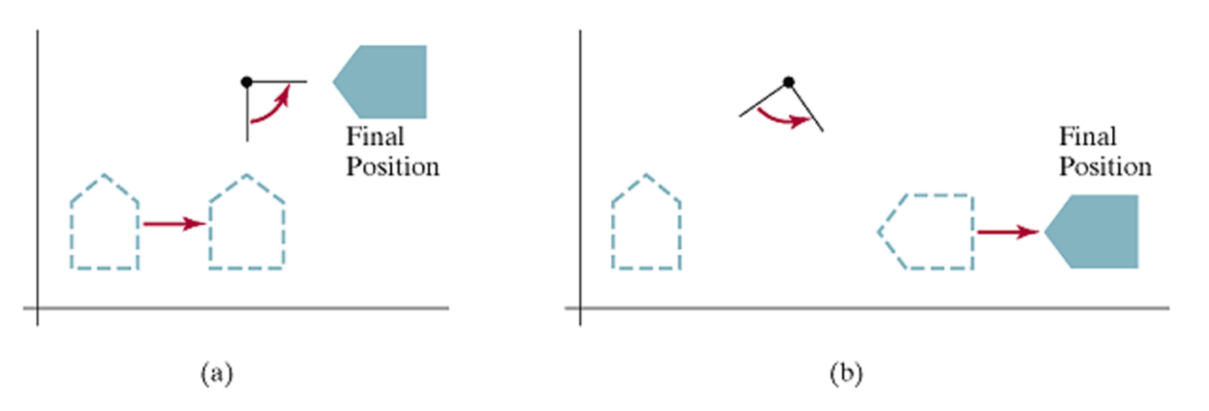
\includegraphics[width=0.8\textwidth]{Figures/comutatividade}
			\caption{(a) Há uma translação depois uma rotação - (b) Há uma rotação depois uma translação.}
		\end{center}
	\end{figure}
	
	
\end{frame}


%%%%%%%%%%%%%%%%%%%%%%%%%%%%%%%%%%%%%%%%%%%%%%%%%%%%%%%%%%%%%%%%%%%%%%%%%%%%%%%%%%%%%%%%%%
\begin{frame}
\frametitle{Transformações Compostas}
	\begin{block}{Composição de Duas Translações}
		
			
		\begin{eqnarray*}
			\textbf{P}' = \textbf{T}(t_{2_x},t_{2_y}) \cdot \textbf{T}(t_{1_x},t_{1_y}) \cdot \textbf{P} \\
			\textbf{P}' = \textbf{T}(t_{2_x},t_{2_y}) \cdot \{\textbf{T}(t_{1_x},t_{1_y}) \cdot \textbf{P} \} \\
			\textbf{P}' = \{\textbf{T}(t_{2_x},t_{2_y}) \cdot \textbf{T}(t_{1_x},t_{1_y}) \} \cdot \textbf{P}  \\
			\begin{bmatrix}
					1	& 0 	& t_{1_x} \\
					0 	& 1	& t_{1_y} \\
					0	& 0	& 1
			\end{bmatrix}
			\cdot \begin{bmatrix}
					1	& 0 	& t_{2_x} \\
					0 	& 1	& t_{2_y} \\
					0	& 0	& 1
			\end{bmatrix}
			= \begin{bmatrix}
					1	& 0 	& t_{1_x} + t_{2_x} \\
					0 	& 1	& t_{1_y} + t_{2_y}\\
					0	& 0	& 1
			\end{bmatrix}
		\end{eqnarray*}
				

	\end{block}
\end{frame}


%%%%%%%%%%%%%%%%%%%%%%%%%%%%%%%%%%%%%%%%%%%%%%%%%%%%%%%%%%%%%%%%%%%%%%%%%%%%%%%%%%%%%%%%%%
\begin{frame}
\frametitle{Transformações Compostas}
	\begin{block}{Composição de Duas Rotações}
		
			
		\begin{eqnarray*}
			\textbf{P}' = \textbf{R}(\theta_1) \cdot \textbf{R}(\theta_2) \cdot \textbf{P} \\
			\textbf{P}' = \textbf{R}(\theta_1) \cdot \{\textbf{R}(\theta_2) \cdot \textbf{P} \} \\
			\textbf{P}' = \{\textbf{R}(\theta_1) \cdot \textbf{R}(\theta_2) \} \cdot \textbf{P}  \\
			\begin{bmatrix}
					cos(\theta_1)	& -sen (\theta_1) 	& 0 \\
					sen(\theta_1) 	& cos(\theta_1)	& 0 \\
					0	& 0	& 1
			\end{bmatrix}
			\cdot \begin{bmatrix}
					cos(\theta_2)	& -sen (\theta_2) 	& 0 \\
					sen(\theta_2) 	& cos(\theta_2)		& 0 \\
					0	& 0	& 1
			\end{bmatrix} \\
			= \begin{bmatrix}
					cos(\theta_1 +\theta_2)	& -sen (\theta_1 +\theta_2) 	& 0 \\
					sen(\theta_1 +\theta_2) 	& cos(\theta_1 +\theta_2)	& 0 \\
					0	& 0	& 1
			\end{bmatrix}
		\end{eqnarray*}
				

	\end{block}
\end{frame}

%%%%%%%%%%%%%%%%%%%%%%%%%%%%%%%%%%%%%%%%%%%%%%%%%%%%%%%%%%%%%%%%%%%%%%%%%%%%%%%%%%%%%%%%%%
\begin{frame}
\frametitle{Transformações Compostas}
	\begin{block}{Composição de Duas Escalas}
		
			
		\begin{eqnarray*}
			\textbf{P}' = \textbf{S}(s_{x_2},s_{y_2}) \cdot \textbf{S}(s_{x_1},s_{y_1}) \cdot \textbf{P} \\
			\textbf{P}' = \textbf{S}(s_{x_2},s_{y_2}) \cdot \{ \textbf{S}(s_{x_1},s_{y_1}) \cdot \textbf{P} \} \\
			\textbf{P}' = \{ \textbf{S}(s_{x_2},s_{y_2}) \cdot \textbf{S}(s_{x_1},s_{y_1}) \} \cdot \textbf{P} \\
			\begin{bmatrix}
					s_{x_2}	& 0 			& 0 \\
					0 		& s_{y_2}	& 0 \\
					0		& 0			& 1
			\end{bmatrix}
			\cdot \begin{bmatrix}
					s_{x_1}	& 0 			& 0 \\
					0 		& s_{y_1}	& 0 \\
					0		& 0			& 1
			\end{bmatrix}
			= \begin{bmatrix}
					s_{x_1}\cdot s_{x_2} 	& 0 						& 0 \\
					0 					& s_{y_1}\cdot s_{y_2}	& 0 \\
					0					& 0						& 1
			\end{bmatrix}
		\end{eqnarray*}
				

	\end{block}
\end{frame}


%%%%%%%%%%%%%%%%%%%%%%%%%%%%%%%%%%%%%%%%%%%%%%%%%%%%%%%%%%%%%%%%%%%%%%%%%%%%%%%%%%%%%%%%%%
\begin{frame}
\frametitle{Transformações Compostas}
	\begin{block}{Rotação 2D Com Ponto de Rotação}
		\begin{itemize}
			\item Este tipo de transformação é feita utilizando várias transformações:
				\begin{itemize}
					\item Translada-se o ponto de referência do objeto à origem.
					\item Aplica-se a transformação de rotação.
					\item Translada-se o ponto de referência do objeto para a origem.
				\end{itemize}
		\end{itemize}						

	\end{block}
	
\end{frame}


%%%%%%%%%%%%%%%%%%%%%%%%%%%%%%%%%%%%%%%%%%%%%%%%%%%%%%%%%%%%%%%%%%%%%%%%%%%%%%%%%%%%%%%%%%
\begin{frame}
\frametitle{Transformações Compostas}
	
	\begin{block}{Em Notação Matricial }
		
		\begin{eqnarray*}
			\textbf{P}' = \textbf{R}(x_r,x_r,\theta) \cdot \textbf{P} \\
			\textbf{R}(x_r,x_r,\theta) = \textbf{T}(\Delta x,\Delta y) \cdot \textbf{R}(\theta) \cdot \textbf{T}^{-1}( \Delta x,\Delta y)
			\end{eqnarray*}
	\end{block}	
	
	\begin{block}{$\textbf{R}(x_r,x_r,\theta)$ Em Notação Matricial }
		
		\begin{eqnarray*}
			\begin{bmatrix}
					1	& 0 	& \Delta x \\
					0 	& 1	& \Delta y \\
					0	& 0	& 1
			\end{bmatrix}
			\cdot \begin{bmatrix}
					cos(\theta)	& -sen (\theta) 	& 0 \\
					sen(\theta) 	& cos(\theta)		& 0 \\
					0	& 0	& 1
			\end{bmatrix}
			\cdot \begin{bmatrix}
					1	& 0 	& -\Delta x \\
					0 	& 1	& -\Delta y \\
					0	& 0	& 1
			\end{bmatrix}\\
			=  \begin{bmatrix}
					cos(\theta)	& -sen(\theta) & x_r-x_r \cdot cos(\theta)+y_r \cdot sen(\theta) \\
					sen(\theta) & cos(\theta)	& y_r-y_r \cdot cos(\theta)-x_r \cdot sen(\theta) \\
					0	& 0	& 1
			\end{bmatrix}
		\end{eqnarray*}
	\end{block}
\end{frame}

%%%%%%%%%%%%%%%%%%%%%%%%%%%%%%%%%%%%%%%%%%%%%%%%%%%%%%%%%%%%%%%%%%%%%%%%%%%%%%%%%%%%%%%%%%
\begin{frame}
\frametitle{Transformações Compostas}
	
	\begin{figure}[!h]
		\begin{center}
			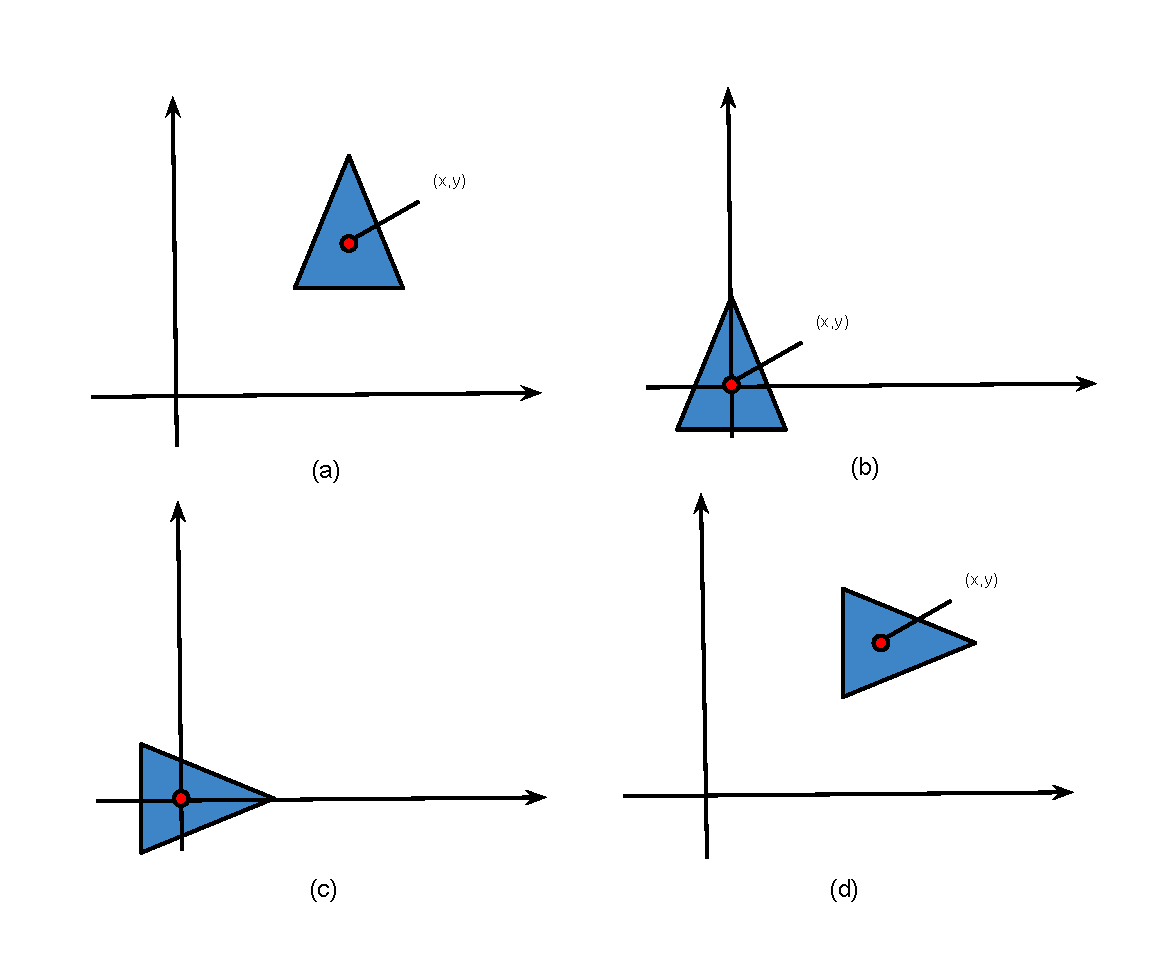
\includegraphics[width=0.6\textwidth]{Figures/RotacaoPontoFixo}
			\caption{Passos para efetuar rotação em torno de um ponto referencial.}
		\end{center}
	\end{figure}
	
\end{frame}

%%%%%%%%%%%%%%%%%%%%%%%%%%%%%%%%%%%%%%%%%%%%%%%%%%%%%%%%%%%%%%%%%%%%%%%%%%%%%%%%%%%%%%%%%%
\begin{frame}
\frametitle{Transformações Compostas}
	\begin{block}{Escala 2D com Ponto de Referência}
		\begin{itemize}
			\item Utiliza-se várias transformações para efetuar a escala:
				\begin{itemize}
					\item Translada-se o ponto de referência do objeto à origem.
					\item Aplica-se a transformação de escala.
					\item Translada-se o ponto de referência do objeto para a origem.
				\end{itemize}
		\end{itemize}						

	\end{block}
	
	

\end{frame}		



%%%%%%%%%%%%%%%%%%%%%%%%%%%%%%%%%%%%%%%%%%%%%%%%%%%%%%%%%%%%%%%%%%%%%%%%%%%%%%%%%%%%%%%%%%
\begin{frame}
\frametitle{Transformações Compostas}
		
		\begin{block}{Em Notação Matricial }
		\begin{eqnarray*}
			\textbf{P}' = \textbf{S}(x_f,y_f,s_x,s_y) \cdot \textbf{P} \\
			\textbf{S}(x_f,y_f,s_x,s_y) = \textbf{T}(x_f,y_f) \cdot \textbf{S}(s_x,s_y) \cdot \textbf{T}^{-1}(x_f,y_f)
		\end{eqnarray*}
		\end{block}		
		
		\begin{block}{$\textbf{S}(x_f,y_f,s_x,s_y)$ Em Notação Matricial }
		
		\begin{eqnarray*}
			\begin{bmatrix}
					1	& 0 	& x_f \\
					0 	& 1	& y_f \\
					0	& 0	& 1
			\end{bmatrix}
			\cdot \begin{bmatrix}
					s_x	& 0 		& 0 \\
					0 	& s_y	& 0 \\
					0	& 0		& 1
			\end{bmatrix}
			\cdot \begin{bmatrix}
					1	& 0 	& -x_f \\
					0 	& 1	& -y_f \\
					0	& 0	& 1
			\end{bmatrix}
			=  \begin{bmatrix}
					s_x	& 0 		& x_f(1-s_x) \\
					0 	& s_y	& y_f(1-s_y) \\
					0	& 0		& 1
			\end{bmatrix}
		\end{eqnarray*}
	\end{block}
		
\end{frame}	


%%%%%%%%%%%%%%%%%%%%%%%%%%%%%%%%%%%%%%%%%%%%%%%%%%%%%%%%%%%%%%%%%%%%%%%%%%%%%%%%%%%%%%%%%%
\begin{frame}
\frametitle{Transformações Compostas}
		
	\begin{figure}[!h]
		\begin{center}
			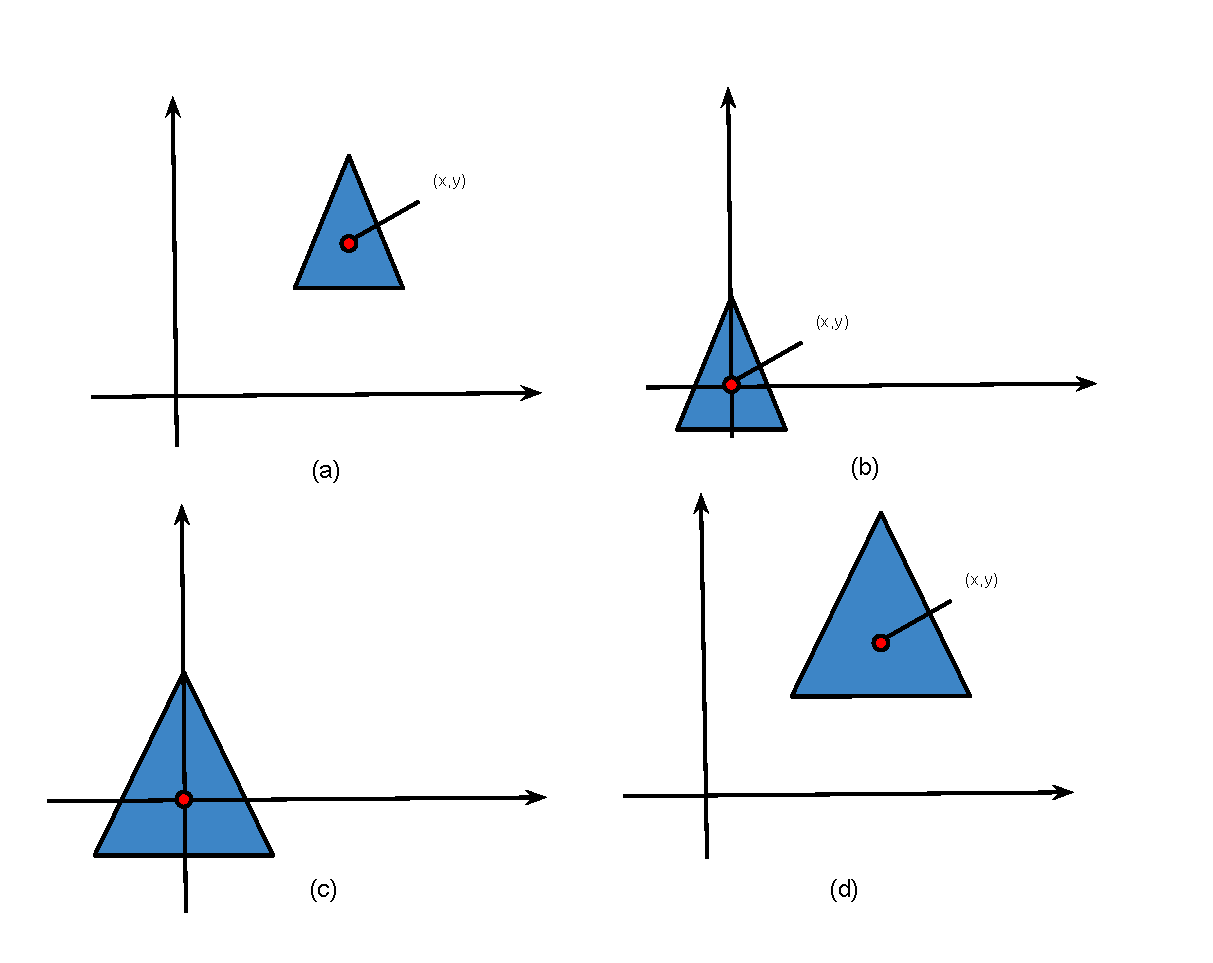
\includegraphics[width=0.6\textwidth]{Figures/EscalaPontoFixo}
			\caption{Passos para efetuar escala em torno de um ponto referencial.}
		\end{center}
	\end{figure}
		
\end{frame}	

%%%%%%%%%%%%%%%%%%%%%%%%%%%%%%%%%%%%%%%%%%%%%%%%%%%%%%%%%%%%%%%%%%%%%%%%%%%%%%%%%%%%%%%%%%
\begin{frame}
\frametitle{Transformações Compostas}
	\begin{block}{Escala em Direções Gerais}
		
		\begin{itemize}
			\item Os tipos de escalas apresentadas até agora apenas escalam em x e y.
			\item Para efetuar escalas em direções gerais é necessário:
			\item Rotacionar o objeto.
			\item Escalar o objeto.
			\item Rotacionar novamente.
		\end{itemize}
	\end{block}
	
	\begin{block}{Em Notação Matricial}
		$\textbf{S}(s_1,s_2,\theta) = \textbf{R}^{-1}(\theta) \cdot \textbf{S}(s_1,s_2) \cdot \textbf{R}(\theta)$ 
	\end{block}
		
\end{frame}	

%%%%%%%%%%%%%%%%%%%%%%%%%%%%%%%%%%%%%%%%%%%%%%%%%%%%%%%%%%%%%%%%%%%%%%%%%%%%%%%%%%%%%%%%%%
\begin{frame}
\frametitle{Transformações Compostas}

	\begin{figure}[!h]
		\begin{center}
			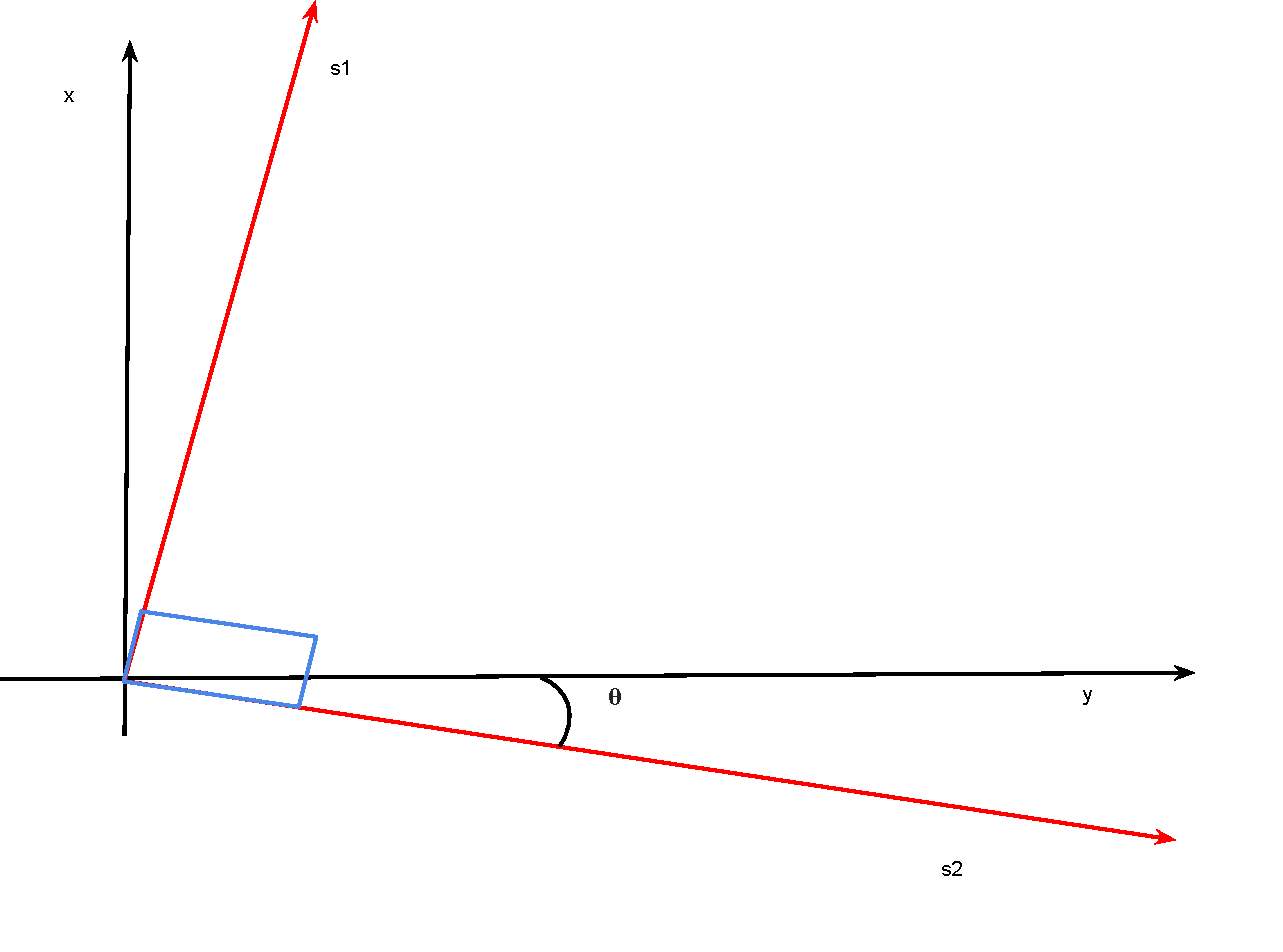
\includegraphics[width=0.6\textwidth]{Figures/escalaGeral}
		\end{center}
	\end{figure}
		
\end{frame}	

%%%%%%%%%%%%%%%%%%%%%%%%%%%%%%%%%%%%%%%%%%%%%%%%%%%%%%%%%%%%%%%%%%%%%%%%%%%%%%%%%%%%%%%%%%
\begin{frame}
\frametitle{Transformações Compostas}

	\begin{figure}[!h]
		\begin{center}
			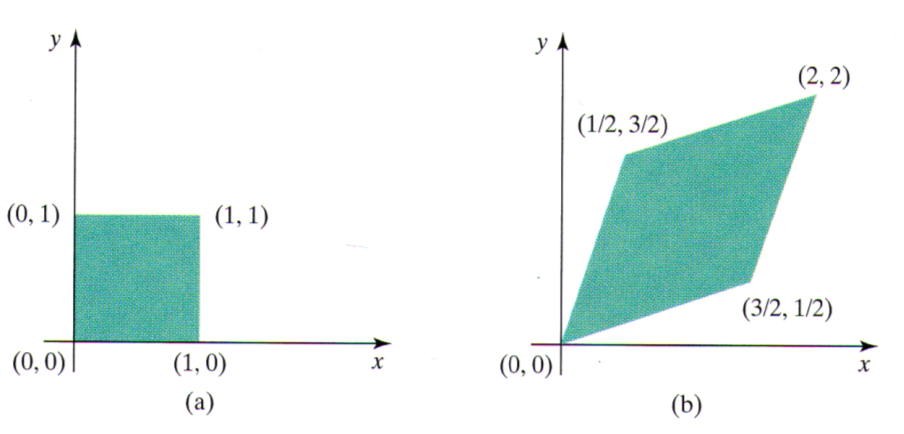
\includegraphics[width=0.9\textwidth]{Figures/EscalaGeralEx}
			\caption{Transformação com $s_1=1,s_2=2$ e $\theta = 45^{\circ}$}
		\end{center}
	\end{figure}
		
\end{frame}	

%%%%%%%%%%%%%%%%%%%%%%%%%%%%%%%%%%%%%%%%%%%%%%%%%%%%%%%%%%%%%%%%%%%%%%%%%%%%%%%%%%%%%%%%%%
\section{Outros Tipos de Transformações}
\subsection{Reflexão}
\begin{frame}
\frametitle{Outros Tipos de Transformações}
	\begin{block}{Reflexão - Espelhamento}
		\begin{itemize}
			\item Espelha-se as coordenadas do objeto de acordo com o eixo a ser espelhado, rotacionando $180^{\circ}$.
		\end{itemize}
	\end{block}
	
	\begin{block}{Reflexão em y = 0}
		\begin{eqnarray*}
			\begin{bmatrix}
				1 & 0 & 0 \\
				0 & -1 & 0 \\
				0 & 0 & 1 
			\end{bmatrix}
		\end{eqnarray*}
	\end{block}	
	
\end{frame}	

%%%%%%%%%%%%%%%%%%%%%%%%%%%%%%%%%%%%%%%%%%%%%%%%%%%%%%%%%%%%%%%%%%%%%%%%%%%%%%%%%%%%%%%%%%
\begin{frame}
\frametitle{Outros Tipos de Transformações}

	\begin{block}{Reflexão em x = 0}
		\begin{eqnarray*}
			\begin{bmatrix}
				-1 & 0 & 0 \\
				0 & 1 & 0 \\
				0 & 0 & 1 
			\end{bmatrix}
		\end{eqnarray*}
	\end{block}	
	
	\begin{block}{Reflexão em x = 0 e y = 0}
		\begin{eqnarray*}
			\begin{bmatrix}
				-1 & 0 & 0 \\
				0 & -1 & 0 \\
				0 & 0 & 1 
			\end{bmatrix}
		\end{eqnarray*}
	\end{block}	
	
\end{frame}


%%%%%%%%%%%%%%%%%%%%%%%%%%%%%%%%%%%%%%%%%%%%%%%%%%%%%%%%%%%%%%%%%%%%%%%%%%%%%%%%%%%%%%%%%%
\begin{frame}
\frametitle{Outros Tipos de Transformações}

	\begin{figure}[!h]
		\begin{center}
			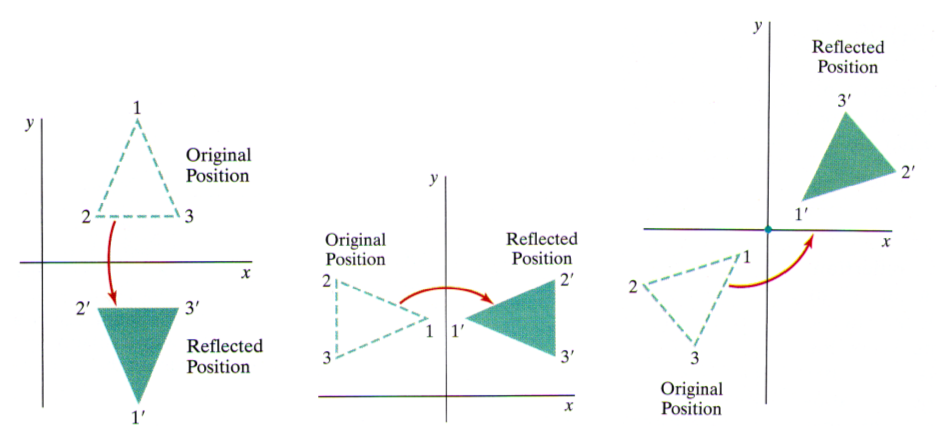
\includegraphics[width=0.9\textwidth]{Figures/reflexo}
		\end{center}
	\end{figure}
		
\end{frame}	

%----------------------------------------------------------------------------------------

\end{document} 